\subsection{NuRV FMU monitor}\label{subsec:NuRVmoni}
NuRV provides the capability to export runtime monitors as standalone FMU components, both for FMI version 2.0 and 3.0. This feature enables users to easily interface monitors within custom applications using a variety of libraries that support the FMU standard.
This section outlines how to utilize these FMU monitors to perform an
early validation of the internal components of the incubator DT before its deployment. Specifically, it is shown how to validate the energy saver and anomaly detection components using an FMU monitor.

\subsubsection{Monitor definition and integration}
The monitor is defined by the SMV model illustrated in \cref{fig:nurv_orbit_spec}. This model specifies a safety LTL property: Whenever an anomaly occurs, the system should reconfigure itself and enter energy-saving mode within a maximum of \texttt{3} time steps. The output of this monitor can be a final verdict of either \textit{true} or \textit{false}, or \textit{unknown} if there is insufficient information to reach a definitive conclusion.
%
\begin{figure}[ht]
	\centering
	\begin{lstlisting}
MODULE main
VAR
    anomaly : boolean;
    energy_saving : boolean;
LTLSPEC -- Safety
    G (anomaly -> F [ 0, 3 ] energy_saving)
	\end{lstlisting}
	\caption{NuRV monitor model}
	\label{fig:nurv_orbit_spec}
\end{figure}%
%
\subsubsection{Simulation environment}
For the validation process, a simulation environment was established
comprising several components (depicted in Fig.~\ref{fig:nurv_fmi_simulation}): the \textit{energy saver} and \textit{anomaly detection} components, each encapsulated within distinct FMUs, along with the NuRV monitor, exported by NuRV using the specification in Fig.~\ref{fig:nurv_orbit_spec}. The input data for the simulation is generated by a purpose-built FMU component named \textit{source}, which supplies testing data to the anomaly detection, simulating an anomaly occurring at time \texttt{t=60s}. A final component, \textit{watcher}, is employed to verify whether the energy saver activates in response to an anomaly reported by the anomaly detector. The FMUs for the energy saver and anomaly detector were constructed packaging their Python code using \lstinline{unifmu}\footnote{\url{https://github.com/INTO-CPS-Association/unifmu}}, while the \textit{source} and \textit{watcher} components were generated using \lstinline{OpenModelica}\footnote{\url{https://openmodelica.org/}}. \lstinline{maestro}\footnote{\url{https://github.com/INTO-CPS-Association/maestro}} served as the co-simulation engine.%
%
\begin{figure}[ht]
	\centering
	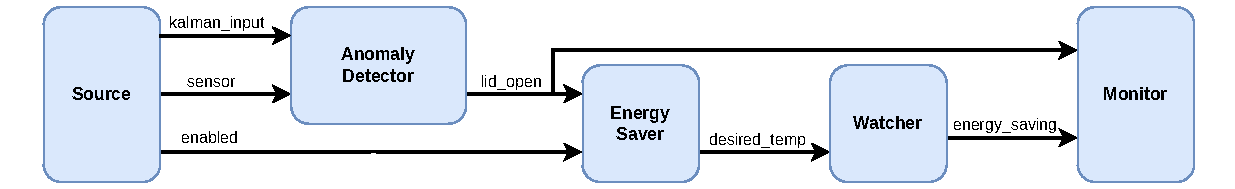
\includegraphics[width=\textwidth]{images/FMI-communication.pdf}
	\caption{Simulation architecture of components and their exchanged signals}
	\label{fig:nurv_fmi_simulation}
\end{figure}%
%
\subsubsection{Simulation creation and execution}
The setup of the simulation is automatically performed through the \texttt{create} script, which installs the required dependencies and compiles the monitor from its specification model. The simulation can then be initiated using the DTaaS \texttt{execute} script, which in turn starts the \textit{maestro} co-simulation engine to simulate the system. Given the characteristics of the FMU monitor exported by NuRV, each invocation of the \textit{doStep} function corresponds to a logical heartbeat of the monitor. This allows the monitor component to assess the current values of its inputs and determine the appropriate outcome, thus providing the user the required information to perform the validation of the components.



\subsection{NuRV FMU service monitor}\label{subsec:NuRVsermoni}
Direct integration of the NuRV FMU monitor into the incubator with its service-oriented architecture is not possible.
However, by implementing straightforward wrapper logic, it becomes viable to expose the FMU as an internal service, thereby enabling its utilization within the DT.
Theoretically, automating this process could be achieved through the development of a dedicated tool; however, no such tool currently exists to the authors' knowledge.
For the purposes of this tutorial, a Python-based prototype has been crafted to demonstrate the potential functionality of such a tool.
It is important to underscore that this solution serves as a prototype only, and certain challenges, such as fault tolerance, remain unaddressed.%
%
\begin{figure}[ht]
	\centering
	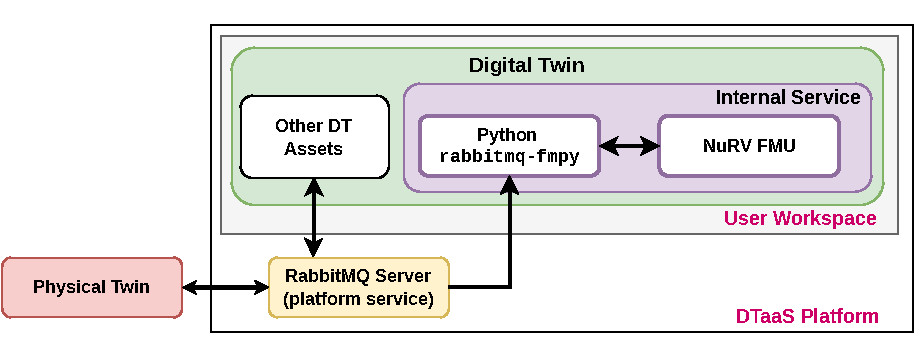
\includegraphics[width=\linewidth]{images/NuRV-FMU-integration.pdf}
	\caption{Overview of components involved with the NuRV FMU service monitor. Notice that \lstinline{rabbitmq} and \lstinline{fmpy} are libraries.}
	\label{fig:nurv-fmu-service}
\end{figure}%
%
\subsubsection{Overview}
As depicted in \cref{fig:nurv-fmu-service}, the tool leverages the Python libraries \lstinline{rabbitmq}\footnote{\url{https://pypi.org/project/rabbitmq/}} and \lstinline{fmpy}\footnote{\url{https://pypi.org/project/FMPy/}}, to realize its functionality.
\lstinline{rabbitmq} facilitates subscription to the RabbitMQ topics that are relevant for the monitor.
\lstinline{fmpy} enables the simulation of an FMU within Python, allowing the introduction of custom logic between each simulation step.
In conjunction, this tool orchestrates its operations such that upon the occurrence of a new message on a topic, the internal state of the Python program is updated, and the signals are subsequently forwarded to the FMU monitor, resulting in the generation of a new verdict.\\
Given the reuse of the FMU, the NuRV specification remains identical to the one outlined previously.

\subsubsection{Creation, execution, and termination}
As an extension of the ``NuRV FMU monitor'' configuration, the prerequisites are a superset of those previously outlined.
Additionally, the Python libraries \lstinline{fmpy} and \lstinline{rabbitmq} must be installed.
As a consequence, the \texttt{create} script fulfills the same function as described above, while also installing the requisite additional Python libraries.\\
In this configuration of the incubator, an additional service in the form of the RV monitor is initiated concurrently with the execution of the DT.
Given that the monitor is deployed as an internal service, it becomes the responsibility of the DT to manage the monitor, thereby intertwining their lifecycles.
Consequently, the \texttt{execute} script commences the DT as usual but with the inclusion of starting the monitor.
This enables the continuous monitoring of the anomaly detection and energy saving blocks, facilitating their verification at runtime.\\
Since the monitor is deployed as an internal service, its lifecycle depends on that of the DT.
As a result, when the purpose of the DT has been met and it is terminated through the \texttt{terminate} script, the monitor is terminated together with it.

\subsection{NuRV ORBit2 monitor}\label{subsec:NuRVORBIT}
% Native DTaaS integration of monitors with orbit
Alternatively, NuRV also facilitates being deployed as a standalone monitoring server service accessible to the DT.
Consequently, the NuRV monitor and DT operate independently, with their lifecycles entirely decoupled from each other.
This section delineates the steps to achieve this with the incubator.

\subsubsection{NuRV monitor server}
NuRV supports a network-based \textit{monitoring server} mode: from the interactive shell mode, NuRV can enter with a command into a network listening state. This enables user code to remotely execute the heartbeat command for online monitoring.
In server mode, NuRV has the capability to accommodate multiple clients connecting to multiple servers. In this context, each \textit{monitor server} refers to a running NuRV process where numerous LTL properties are incorporated alongside their respective runtime monitors, established through the \texttt{build\_monitor} command. It should be emphasized that a single NuRV process has the capacity to administer multiple monitors, each tailored to different LTL properties.


\subsubsection{Monitor integration}
The process of connecting the monitor server to the DT of the incubator is automated by the \texttt{execute} script. This script, in turn, employs a Python script file, that initially launches the \texttt{omniNames} CORBA Name Service utility from the \textit{omniORB} toolset, followed by starting the \texttt{NuRV\_orbit} version of NuRV. Subsequently, a connection is established with the monitor server using the \textit{omniORB} Python library. Once this connection is established, the Python script starts the incubator DT and subscribes to relevant RabbitMQ topics such as energy saver status and lid open status. The lid open status will be mapped to the anomaly for the NuRV monitor.\\
Fig.~\ref{fig:nurv-orbit-architecture-diagram} shows the architecture of the system comprising the incubator DT and the NuRV monitoring server.%
%
\begin{figure}[ht]
	\centering
	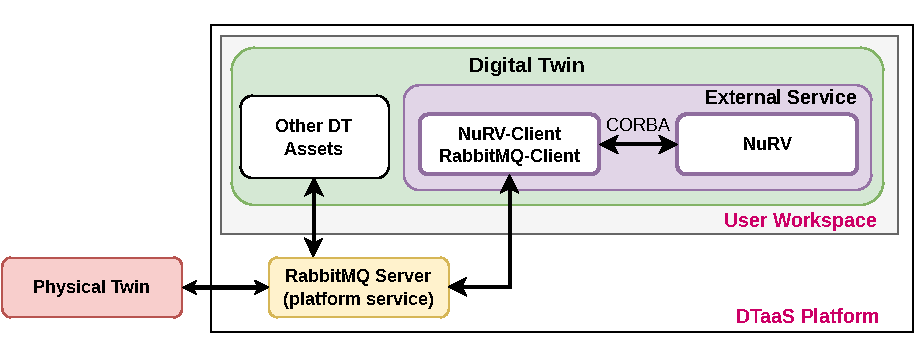
\includegraphics[width=\linewidth]{images/NuRV-native-integration.pdf}
	\caption{Overview of components involved with the NuRV ORBit2 monitor.}
	\label{fig:nurv-orbit-architecture-diagram}
\end{figure}
%
Upon receiving a message, the DT's status is relayed to NuRV via a heartbeat operation call through the CORBA interface. NuRV responds to this heartbeat by providing the monitor's output. If the monitor's output represents a final verdict, the monitor is reset to prepare for its utilisation for the subsequent execution of the DT.
